%\begin{savequote}[75mm]
%Nulla facilisi. In vel sem. Morbi id urna in diam dignissim feugiat. Proin molestie tortor eu velit. Aliquam erat volutpat. Nullam ultrices, diam tempus vulputate egestas, eros pede varius leo.
%\qauthor{Quoteauthor Lastname}
%\end{savequote}

\chapter{{\it Prelude}: on numerical techniques}
\label{ch:numerics}

\epigraph{In collaboration with A.~Philippov, J.~Mahlmann, D.~Groselj, F.~Bacchini, and A.~Spitkovsky}

Matter around compact astrophysical objects is typically fully ionized. As a result, the dynamics of such matter is vitally governed by the interplay between the charged particles and the electromagnetic field. Complete mathematical description of such system requires consideration of the Boltzmann equation \citep{1981phki.book.....L},

\begin{equation}
  \label{eq:vlasov-maxwell-boltzmann}
  \frac{\partial f_s}{\partial t} + \bm{v} \nabla f_s - \frac{q_s}{m_s}\left(\bm{E}+\frac{\bm{v}}{c}\times\bm{B}\right)\frac{\partial f_s}{\partial \bm{v}} = \left(\frac{\partial f_s}{\partial t}\right)_{\rm col},
\end{equation}
\noindent a time-dependent kinetic equation on the distribution functions of charged particles $f_s(t;\bm{r},\bm{v})$ for a given species $s$. The right-hand-side of this equation is called the Landau collision integral; it describes the evolution of a distribution function due to close encounters of charged particles with each other -- a process also referred to as \emph{Coulomb collisions}. While individual Coulomb collisions occur via electromagnetic interaction and are technically accounted for in the left-hand-side of the equation~\eqref{eq:vlasov-maxwell-boltzmann}, it is useful to distinguish the former from long-range electromagnetic interactions. Then $\bm{E}$ and $\bm{B}$ represent self-consistent electric and magnetic fields created by both the external sources and the collective motion of charged particles of our system.

In practice, for plasmas around compact objects Coulomb collisions occur at much longer timescales than, e.g., particle gyration or acceleration. Such plasma is often called \emph{collisionless}.\footnote{As opposed to collisional plasma, where Coulomb collisions or other short interactions (e.g. wave-particle scattering) effectively thermalize the plasma, making it ``fluid-like''. These plasmas are typically studied by the means of magnetohydrodynamics (MHD; \citealt{1960ecm..book.....L}).} Because of this the right-hand-side of~\eqref{eq:vlasov-maxwell-boltzmann} is neglected in the context of collisionless plasma, and the resulting equation is called \emph{Vlasov equation} \citep{1968SvPhU..10..721V}. 


This formula then has to be coupled with Maxwell's equations on electromagnetic fields, $\bm{E}(t;\bm{r})$ and $\bm{B}(t;\bm{r})$:

\begin{multicols}{2}
  \begin{equation}
    \label{eq:faraday-law}
    \frac{1}{c}\frac{\partial \bm{B}}{\partial t} = -\nabla \times\bm{E},
  \end{equation}
  \begin{equation}
    \label{eq:ampere-law}
    \frac{1}{c}\frac{\partial \bm{E}}{\partial t} = \nabla \times\bm{B} - \frac{4\pi}{c}\bm{j},
  \end{equation}
\end{multicols}
\noindent where for a closed system the current, $\bm{j}$, is self-consistently regulated by the motion of individual particles:

\begin{equation}
  \label{eq:current-density}
  \bm{j} = \sum_s q_s \int \bm{v} f_s \mathrm{d}^3\bm{v}.
\end{equation}

Notice that we essentially formulate an initial-value problem with a set of hyperbolic evolution equations \eqref{eq:vlasov-maxwell-boltzmann}, \eqref{eq:faraday-law}, and \eqref{eq:ampere-law} coupled via closure expression \eqref{eq:current-density}. If the initial conditions satisfy the two remaining Maxwell's equations at a certain initial time $t=t_0$, it can be easily demonstrated that the solution to the former set of equations will also satisfy the latter. Thus we can only consider the other two Maxwell's equations as initial conditions

\begin{multicols}{2}
  \begin{equation}
    \label{eq:poisson-law}
    \nabla\cdot \bm{E} = 4\pi \rho,
  \end{equation}
  \begin{equation}
    \label{eq:divb-law}
    \nabla\cdot \bm{B} = 0,
  \end{equation}
\end{multicols}
\noindent where $\rho$ is the charge density defined similar to the current density in equation \eqref{eq:current-density}:

\begin{equation}
  \label{eq:charge-density}
  \rho = \sum_s q_s \int f_s \mathrm{d}^3 \bm{v}.
\end{equation}

Due to its non-linear coupling the equation set \eqref{eq:vlasov-maxwell-boltzmann} - \eqref{eq:current-density} has no general solution, and in most of the interesting cases has to be studied numerically. In practice, numerically solving this system, even when discretized in phase space and time, proves highly expensive computationally, as the discretization has to be performed in a 6+1 dimensional space, and the computational cost thus scales as the resolution to the sixth power. There are various approaches and assumption that help reduce the complexity of the problem, one of which -- \emph{the particle-in-cell (PIC) algorithm} -- I employ in my work.

\section{Particle-in-cell algorithm for kinetic plasma simulations}
\label{sec:pic}

In PIC algorithm \citep{1986ITPS...14..661B, 1991ppcs.book.....B} instead of discretizing the phase space, the distribution function itself is sampled with a finite number of \emph{macro-particles} each having a continuous value for the coordinate and velocity. Thus, at a given moment in time the distribution function can be expressed as

\begin{equation}
  \label{eq:pic-df}
  f_s(t;\bm{r},\bm{v}) = \sum_p w_{s,p}S\left(\bm{r} - \bm{r}_{s,p}(t)\right)\delta\left(\bm{v}-\bm{v}_{s,p}(t)\right),
\end{equation}
\noindent where $\bm{r}_{s,p}(t)$ and $\bm{v}_{s,p}(t)$ are the coordinate and the velocity of the $p$-th macro-particle of species $s$, while $w_{s,p}$ is the effective weight. Function $S$, which describes smearing of each individual particle, is called \emph{the shape function}. Here and further in this text I will be using the terms ``macro-particle" and ``particle" interchangebly in the context of numerical simulations. We may thus treat each individual particle separately, independendently integrating their equations of motion:

\begin{equation}
  \label{eq:eom}
\begin{aligned}
  \frac{\mathrm{d}\bm{x}_{s,p}}{\mathrm{d}t} &= \bm{v}_{s,p},\\
  \frac{\mathrm{d}\bm{u}_{s,p}}{\mathrm{d}t} &= \frac{1}{m_s}\bm{F}_{s,p},\\
\end{aligned}
\end{equation}
\noindent where $\bm{F}_{s,p}$ is the sum of all forces acting on the given particle, and $\bm{u}_{s,p}$ is the spatial component of the particle four-velocity: $\bm{u}_{s,p} = \bm{v}_{s,p}\gamma_{s,p}$ ($\gamma_{s,p}$ is the particle \emph{Lorentz factor}). In our case, $\bm{F}_{s,p}$ will be the Lorentz force generated by the collective electromagnetic field.

Electric and magnetic fields, on their turn, are discretized spatially -- $\bm{E}_{i,j,k}$ and $\bm{B}_{i,j,k}$ -- where $i,j,k$ is the three-dimensional index of the corresponding node in the discretized space. In the present discussion we will consider discretization on a Cartesian grid, however, more complex cases have also been implemented and are widely used (polar: \citealt{2014ApJ...795L..22C, 2015NewA...36...37B}, spherical: \citealt{2019ascl.soft11012C}, GR: \citealt{2019PhRvL.122c5101P}; here we only mention relativistic PIC codes, while there are numerous other non-relativistic implementations). Coupling between the particles and electromagnetic fields is performed in two ways. First of all, each individual macroparticle deposits currents on the grid: $\bm{j}_{s,p;~i,j,k}$. The deposit algorithm is typically designed to be charge conservative: meaning that the deposited currents satisfy the discretized charge continuity equation:
\begin{equation}
  \label{eq:charge-continuity}
  \frac{\partial \rho}{\partial t} + \nabla\cdot \bm{j} = 0.
\end{equation}
\noindent This discretized current, summed over all species and particles, is then used as a source terms in the Ampere's law~\eqref{eq:ampere-law}, which, together with the Faraday's law~\ref{eq:faraday-law} is used to advance the electric and magnetic fields in time. Electromagnetic fields, on the other hand, act on particles via the Lorentz force
\begin{equation}
  \label{eq:lorentz-force}
  \bm{F}_{s,p} = q_s \left(\bm{E}(\bm{r}_{s,p}) + \frac{\bm{v}_{s,p}}{c}\times \bm{B}(\bm{r}_{s,p})\right),
\end{equation}
\noindent which is then used in the equations of motion for each individual particle~\eqref{eq:eom}, thus closing the algorithm loop.\footnote{Notice that to compute the value for the electric or magnetic field at the position of the particle in~\eqref{eq:lorentz-force}, or to compute the contribution of each individual particle to the discretized current density, interpolation and extrapolation algorithms are typically used which employ the particle shape function, defined in~\eqref{eq:pic-df}.}

To summarize, the key steps of the particle-in-cell algorithm are shown in figure~\ref{fig:pic-steps}. On top of what has already been discussed, we also use a gaussian current filtering (shown as substep (5) in figure~\ref{fig:pic-steps}) to mitigate noise due to the finite number of macroparticles per simulation cell. Typically a \emph{leapfrog time-integration algorithm} is chosen to advance particle positions and velocities (as well as electric and magnetic field components). This ensures the second-order accuracy in time \citep{1991ppcs.book.....B}. However, this also means that the coordinates and velocities of each individual particle (as well as $\bm{E}$ and $\bm{B}$ field components) are staggered in time by half timestep (hence the ``${(n-1/2)}$'' index for velocities and magnetic field components). It is also convenient to define the discretized values of the electromagnetic field components at different locations with respect to the corresponding node $(i,j,k)$. This is the so-called \emph{Yee-mesh configuration} \citep{1966ITAP...14..302Y}. In this case, for instance, $E_{x;~i,j,k}$ corresponds spatially to $E_{x;~i+1/2,j,k}$ (staggered by half cell in the $+x$ direction), however for brevity we typically omit the extra $1/2$ in the index.\footnote{A simple explanation behind this non-trivial convention is that in the integrated form Maxwell's equations operate in terms of the contour integrals of the electric field, $\oint\bm{E}\mathrm{d}\bm{l}$, and the fluxes of the magnetic field, $\oiint \bm{B}\mathrm{d}\bm{s}$. When solving these equations in the discretized space with the Yee-mesh configuration, both of these quantities can be trivially computed from the corresponding staggered field components at the boundaries of the computational cell without interpolation.}

As a result, figure~\ref{fig:pic-steps} represents the full set of discretized equations, sometimes referred to as the electromagnetic PIC algorithm, that approximate the solution of the system of hyperbolic equations \eqref{eq:vlasov-maxwell-boltzmann}, \eqref{eq:faraday-law}, and \eqref{eq:ampere-law} coupled via closure \eqref{eq:current-density}. As it was mentioned above, this numerical solution is second-order accurate in time, and converges to analytic solution as long as the timestep is short: $c\Delta t<0.5\Delta x$ ($\Delta x$ is the size of the cell which is typically the same in all dimensions). This is also called a \emph{Courant–Friedrichs–Lewy condition}. Notice also, that these equations locally preserve the charge and $\nabla\cdot\bm{B}$, as well as the spatial components of the total four-momentum (computed for fields and particles). However, due to its explicit nature, the total energy is only conserved up to second order in $\Delta t$.

\begin{figure}[tb]
  \centering
\begin{tikzpicture}[node distance=1cm, auto,]
  \node[box,xshift=2cm] (1) {
      (1) Faraday's law (first half-step):
      \begin{equation*}
        \bm{B}^{(n)} = \bm{B}^{(n-1/2)} -c\nabla\times\bm{E}^{(n)}\frac{\Delta t}{2}.
      \end{equation*}
    };
  \node[box,below right=of 1,xshift=-2cm,yshift=-2cm] (3) {
      (3) Particle EOM integration:
      \begin{equation*}
      \begin{aligned}
        \bm{u}_{s,p}^{(n+1/2)} = \bm{u}_{s,p}^{(n-1/2)} + \Delta t \bm{F}_{s,p}/m_s,\\
        \bm{r}_{s,p}^{(n+1)} = \bm{r}_{s,p}^{(n)} + \Delta t \bm{v}_{s,p}^{(n+1/2)}.
      \end{aligned}
      \end{equation*}
    };
  \node[box,below=of 3,yshift=-2cm,xshift=-2cm] (4) {
      (4) Current deposition:
      \begin{equation*}
        \bm{r}_{s,p}^{(n+1)}, \bm{v}_{s,p}^{(n+1/2)}\rightarrow \bm{j}^{(n+1/2)}_{i,j,k}.
      \end{equation*}
    };
  \node[box,above left=of 4,yshift=0.5cm,xshift=2cm] (6) {
      (6) Faraday's law (second half-step):
      \begin{equation*}
        \bm{B}^{(n+1/2)} = \bm{B}^{(n)} - c\nabla\times \bm{E}^{(n)}\frac{\Delta t}{2}.
      \end{equation*}
    };
  \node[box,above=of 6] (7) {
      (7) Ampere's law:
      \begin{multline*}
        \bm{E}^{(n+1)} = \bm{E}^{(n)} + c\nabla\times \bm{B}^{(n+1/2)}\Delta t \\- 4\pi \tilde{\bm{j}}^{(n+1/2)}\Delta t.
      \end{multline*}
    };
  \draw[arrow] (1) to[bend left=20]
    node [float,midway,align=left,yshift=-0.3cm,xshift=0cm] {
      (2) Interpolation of the Lorentz force onto particles: \\
      $\bm{E}_{i,j,k}^{(n)},~\bm{B}_{i,j,k}^{(n)}\rightarrow \bm{E}(\bm{r}_{s,p}),~\bm{B}(\bm{r}_{s,p}),$
      $\bm{E}(\bm{r}_{s,p}),~\bm{B}(\bm{r}_{s,p})\rightarrow \bm{F}_{s,p}.$
    }
    (3);
  \draw[arrow] (3) to[bend left=20] (4);
  \draw[arrow] (4) to[bend left=10]
    node [float,midway,align=right,yshift=0.3cm,xshift=0cm] {
      (5) Current filtering:
      $\bm{j}^{(n+1/2)}_{i,j,k}\rightarrow \tilde{\bm{j}}^{(n+1/2)}_{i,j,k}.$
    }
    (6);
  \draw[arrow] (6) to (7);
  \draw[arrow] (7) to[bend left=10]
    node [font=\footnotesize,midway,yshift=-0.2cm,align=right] {
      $n\to n+1$
    }
    (1);
\end{tikzpicture}
  \caption{Key steps of the particle-in-cell plasma simulation algorithm.\label{fig:pic-steps}}
\end{figure}

There are numerous implementations of this algorithm. In particular, \texttt{Tristan-MP} \citep{2005AIPC..801..345S} has long been a reliable code widely used by the relativistic plasma astrophysics community. It is written in \texttt{Fortran} and parallelized using the \texttt{MPI} library. \texttt{Tristan-MP v2} \citep{tristanv2} is the new incarnation of the original code with various added capabilities and optimizations. I will discuss some of the new capabilities, such as the radiation and quantum electrodynamic effects, in one of the following sections. Meanwhile, in the following section I describe another important advancement in the new code, aimed to help simulate plasmas in global astrophysical systems, where physically relevant scales are separated by many orders of magnitudes.

%\begin{figure}
  %\centering
  %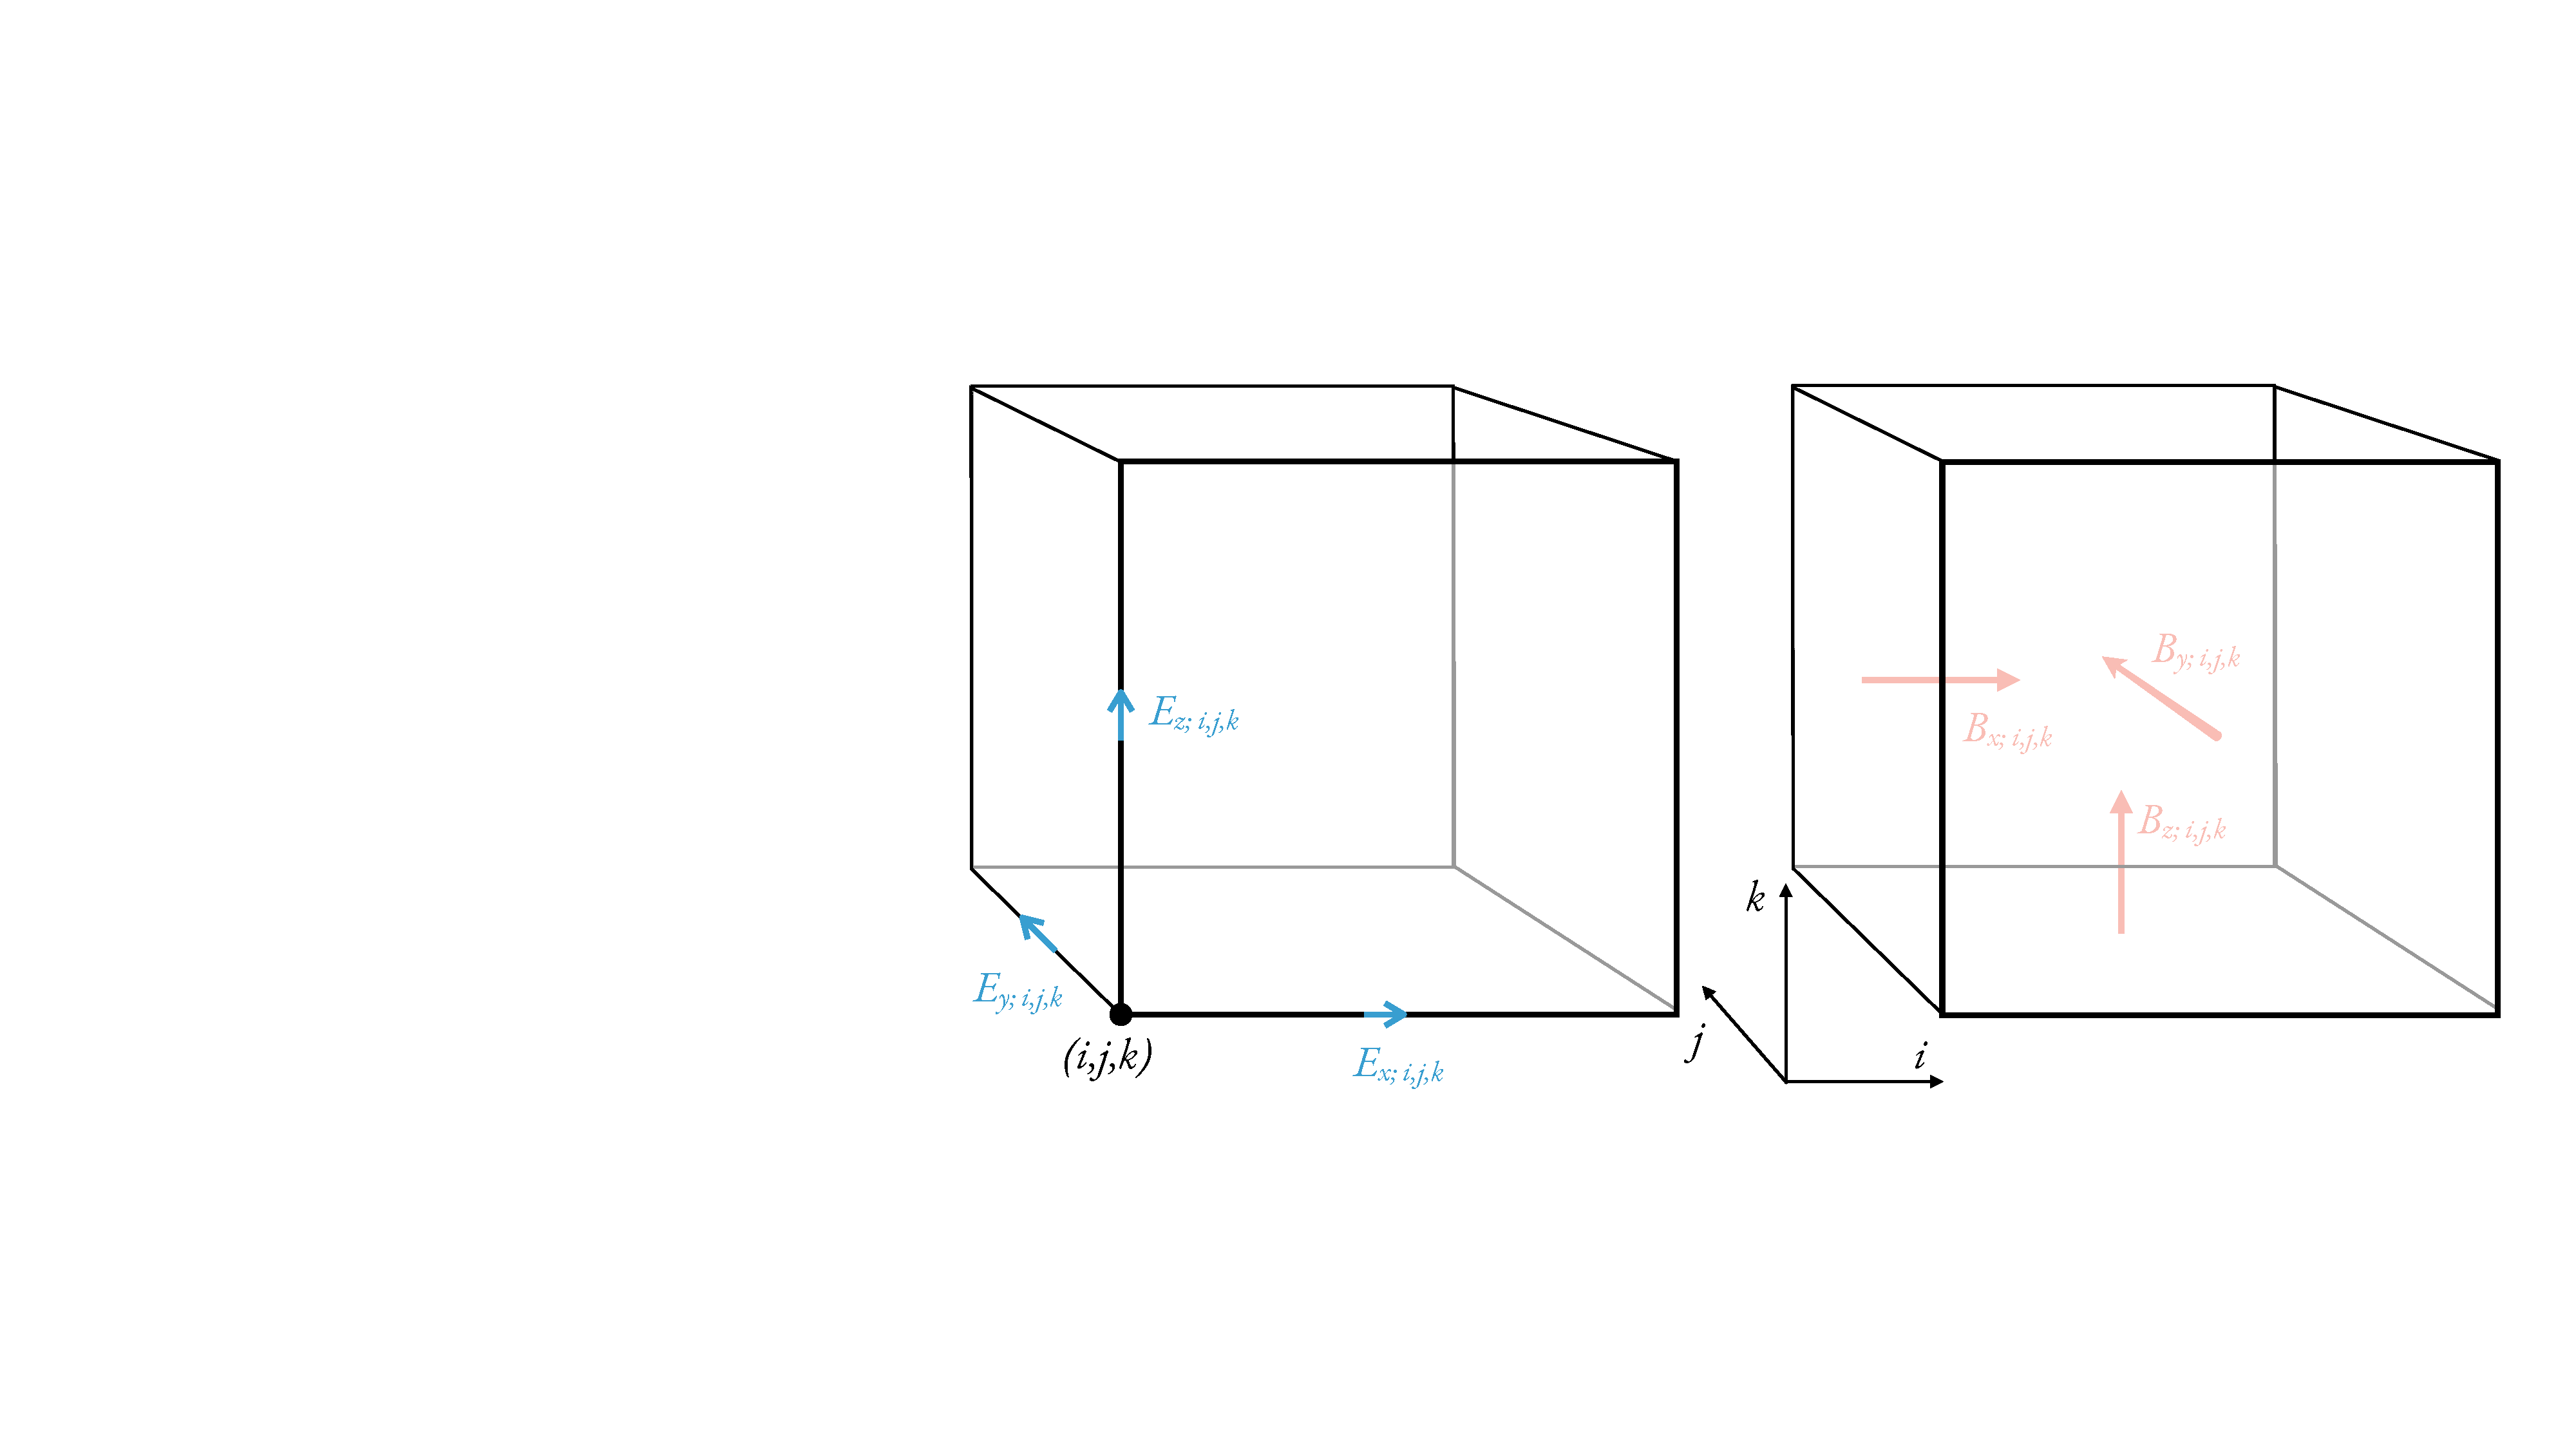
\includegraphics[trim=720 250 20 250,clip,width=0.7\textwidth]{figures/ch1-yee-mesh}
  %\caption[Yee mesh.]{Yee lattice configuration for the discretization of the electromagnetic field components. \label{fig:ch1-yee}}
%\end{figure}

\section{Highly magnetized (guiding center) approximation}
\label{sec:num-gca-approx}

One of the main bottlenecks on the performance of the codes that employ PIC algorithms is the integration of particles' equations of motion (step 3 in figure~\ref{fig:pic-steps}); sometimes also called a \emph{particle push} substep. This integration is typically done using an explicit scheme with several substeps:

\begin{align}
  \bm{r}^{(n+1/2)} &= \bm{r}^{(n)} + \frac{\bm{u}^{(n)}}{2\gamma^{(n)}}\Delta t,\\
  \frac{\bm{u}^{(n+1)}-\bm{u}^{(n)}}{\Delta t} &= \frac{1}{m_s} \bm{F}_{s,p}^{(n+1/2)},\label{eq:part-push2}\\
  \bm{r}^{(n+1)} &= \bm{r}^{(n+1/2)} + \frac{\bm{u}^{(n+1)}}{2\gamma^{(n+1)}}\Delta t.
\end{align}

\noindent Notice, that the Lorentz force, $\bm{F}_{s,p}$, in this scheme shall contain the particle's velocity \eqref{eq:lorentz-force}. In general, equation \eqref{eq:part-push2} is implicit with respect to the $\bm{u}^{(n+1)}$. However, typically, explicit approach is used for solving it. One of the most commonly used ones is the \emph{Boris algorithm} \citep{Boris1970}, which is performed in three substeps:
\begin{equation}
\label{eq:num-boris}
  \begin{aligned}
    \textrm{half electric acceleration:  }&\bm{u}^- = \bm{u}^{(n)} + \frac{q_s}{m_s}\bm{E}(\bm{r}^{(n+1/2)})\frac{\Delta t}{2}, \\
    \textrm{magnetic rotation:  }& \bm{u}^+  = \bm{u}^- + (\bm{u}^-+\bm{u}^-\times \bm{t})\times\bm{s},\\
    \textrm{half electric acceleration:  }&\bm{u}^{(n+1)} = \bm{u}^+ + \frac{q_s}{m_s}\bm{E}(\bm{r}^{(n+1/2)})\frac{\Delta t}{2}.
  \end{aligned}
\end{equation}

\noindent Here $\bm{u}^\pm$ are intermediate variables, while
\begin{equation}
  \bm{t} = \frac{q_s}{m_s}\frac{1}{\gamma^\pm }\bm{B}(\bm{r}^{(n+1/2)}) \frac{\Delta t}{2 c}, \textrm{ and } \bm{s} = \frac{2\bm{t}}{1 + |\bm{t}|^2}.
\end{equation}
\noindent $\gamma^\pm$ are the Lorentz factors corresponding to intermediate velocities $\gamma^\pm = \sqrt{1 + (\bm{u}^{\pm})^2}$. Notice that they are equal, $\gamma^+ = \gamma^-$, i.e., the magnetic rotation substep does not modify particle's energy.\footnote{This result makes perfect physical sense as the magnetic field cannot impose work on charged particles.} There are numerous other integration schemes for the equations of motion; for a more detailed comprehensive overview and comparison see \cite{2018ApJS..235...21R}.

The opposite extreme is the case when the particle motion is reduced to the motion of its guiding centers \citep[\emph{guiding center approximation}, GCA; see, e.g.,][]{1963RvGSP...1..283N}. This provides a shortcut for systems where gyro-orbits of particles are infinitesimal compared to the macroscopic system size. In this treatment particles are then bound to be carried by magnetic field lines, while the only freedom they are allowed is along the field lines. 

While this approach allows to solve the issue with the scale separation (between gyro-radii and system size), it does not allow to properly capture the plasma dynamics in regions with vanishing magnetic field (e.g., reconnecting current sheets). In \texttt{Tristan-MP v2} we thus employ a hybrid approach introduced by \cite{2020ApJS..251...10B}. This technique allows to couple the conventional Boris algorithm \eqref{eq:num-boris} with the GCA, by ``treating'' particles differently depending on their energy and magnetic fields. For the purposes of studying magnetic reconnection in global pulsar magnetospheres, for instance, particle locations and velocities are updated with a conventional pusher if either of the following criteria is satisfied:

\begin{equation}
    \begin{aligned}
        \gamma\beta \frac{m_s c^2}{|q_s| B} &> f_B \Delta x,\\
        \frac{E}{B} &> f_E.
    \end{aligned}
\end{equation}
\noindent Here $f_B$ and $f_E$ are dimensionless free parameters, typically close to $1$. This criterion states, that unless the particle gyroradius is larger than $f_B\Delta x$ ($\Delta x$ is the size of the simulation cell), or the electric field is larger than $E>f_E B$, its is reduced to that of the guiding center.

As will be demonstrated in one of the future chapters, this technique allows to push the scale separation in simulations closer to realistic astrophysical values. With it we no longer have to resolve gyro-orbits of every individual particle in all of the simulation domain, but rather only focus on properly capturing the dynamics of particles in kinetic regions (where $E_\parallel>B$), while reducing the rest to the motion of their guiding centers. As it is demonstrated in a simple numerical experiment in Figure~\ref{fig:num-gca}, large-scale dynamics, as well as microscopic kinetic properties are largely unaffected by the GCA treatment. 

\begin{figure}[htb]
    \sidebysidecaption{0.7\linewidth}{0.28\linewidth}{
        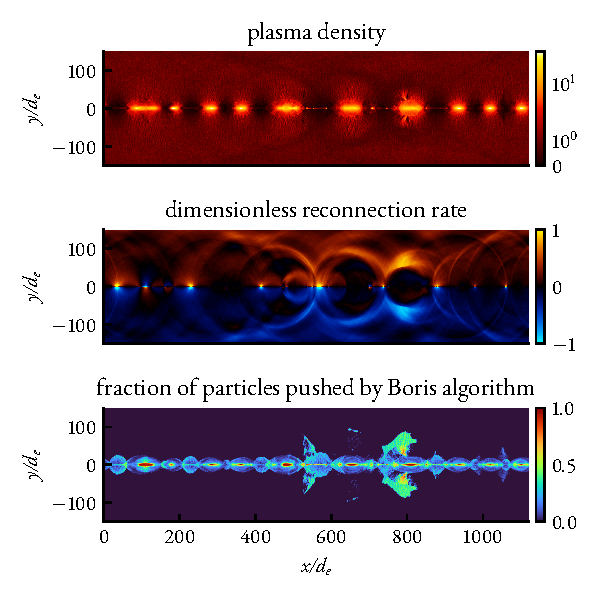
\includegraphics[width=\textwidth]{figures/ch1-numerics/fig_gca.pdf}
    }{
        \caption{A snapshot from the simulation of a 2D relativistic magnetic reconnection where hybrid GCA/Boris particle pusher is used. As shown in the bottom panel, most of the particles (especially in the upstream) are reduced to their guiding centers, and, thus, have no momentum component perpendicular to the magnetic field. Hot current sheets and envelopes around plasmoids are the only regions where particles are energized and switch back to Boris algorithm. Structures of plasmoids, the current sheet, and the reconnection rate are almost identical to runs where no GC approximation is made.}
    \label{fig:num-gca}
    }
\end{figure}

\section{Synchrotron and inverse-Compton cooling}

In the vicinity of compact objects plasma is often ultra-relativistic. In this regime radiative reaction forces may become dynamically important. Typically, this radiation reaction is due to either \emph{synchrotron} radiation in strong magnetic fields, or \emph{inverse-Compton} (IC) radiation induced by a background photon field. While naive PIC simulations do self-consistently capture braking radiation due to accelerated charges, the energy of this radiation is typically orders of magnitude smaller than in reality. Because of that in \texttt{Tristan-MP v2} we introduce an artificial radiation reaction force with an upscaled strength, that can account for both the synchrotron and inverse-Compton cooling.\footnote{For the examples of implementation and usage of similar techniques in PIC simulations see, e.g., \cite{2010NJPh...12l3005T, 2016CoPhC.204..141V, 2016ApJ...828...92Y, 2019ApJ...877...53H, 2019MNRAS.482L..60W, 2020arXiv201203043N}.} This force can be represented in the following form (for a particle with a four-velocity $\bm{u}=\gamma\bm{\beta}$):

\begin{equation}
\begin{split}
\label{eq:num-radiation}
    \bm{f}_{\rm rad} =& \bm{f}_{\rm syn} + \bm{f}_{\rm IC}\\
    =&|q_s| f_{\rm rec} B_{\rm rad}\frac{\bm{\kappa}_R - \gamma^2\chi_R^2 \bm{\beta}}{\gamma_{\rm syn}^2}-|q_s| f_{\rm rec} B_{\rm rad}\frac{\gamma^2}{\gamma_{\rm IC}^2}\bm{\beta}.
\end{split}
\end{equation}
\noindent Here $\kappa_R$ and $\chi_R$ are dimensionless functions of the electric and magnetic field at particle location:

\begin{equation}
    \begin{aligned}
    \label{eq:num-kappa-chi}
        \kappa_R &= \frac{1}{B_{\rm rad}^2}\left[\left(\bm{E} + \bm{\beta}\times\bm{B}\right)\times\bm{B} + (\bm{\beta}\cdot\bm{E})\bm{E}\right],\\
        \chi_R^2 &= \frac{1}{B_{\rm rad}^2}\left[\left(\bm{E} + \bm{\beta}\times\bm{B}\right)^2 - \left(\bm{\beta}\cdot\bm{E}\right)^2\right].
    \end{aligned}
\end{equation}

\noindent Strength of the cooling (either synchrotron or IC) is then parametrized with the choice of fiducial $B_{\rm rad}$\footnote{In the simulations of magnetic reconnection, for instance, $B_{\rm rad}$ is typically chosen to be equal to the background magnetic field strength.} and $f_{\rm rec}$ (which we typically set to $0.1$), and two dimensionless parameters: $\gamma_{\rm syn}$ and $\gamma_{\rm IC}$. These dimensionless parameters quantify the radiation reaction force with respect to the Lorentz force in an electric field of magnitude $f_{\rm rec}B_{\rm rad}$.\footnote{This particular choice is motivated by the fact that in magnetically reconnecting collisionless current sheets with the background magnetic field strength $B$, a resistive electric field is generated of magnitude $f_{\rm rec} B$, where $f_{\rm rec}\approx 0.1$ is the dimensionless reconnection rate (velocity of inflow normalized by the Alfv\'en velocity).} More precisely $\gamma_{\rm syn}$ and $\gamma_{\rm IC}$ are defined in such a way, that:

\begin{equation}
    \begin{aligned}
        |q_e|f_{\rm rec}B_{\rm rad} = 2\sigma_T \frac{B_{\rm rad}^2}{8\pi} \gamma_{\rm syn}^2,\\
        |q_e|f_{\rm rec}B_{\rm rad} = \frac{4}{3}\sigma_T U_{\rm rad} \gamma_{\rm IC}^2.
    \end{aligned}
\end{equation}

\noindent Here $q_e$ is the electron charge, $\sigma_T$ is the Thomson cross section, while $B_{\rm rad}^2/8\pi$ and $U_{\rm rad}$ are the energy densities of the background magnetic field (for synchrotron), and the background photon field (for IC) correspondingly. From \eqref{eq:num-radiation} it is evident, that particles with $\gamma > \gamma_{\rm syn/IC}$ are radiatively cooled at timescales shorter than the acceleration timescale in an electric field of $E=f_{\rm rec}B_{\rm rad}$ via synchrotron/IC mechanism, while the opposite is true for particles with $\gamma < \gamma_{\rm syn/IC}$. 

In practice, during the simulation the radiation reaction force \eqref{eq:num-radiation} is evaluated at every timestep for each particle using the electric and magnetic field values interpolated to particle position, and the particle four-velocity $\bm{u}^{(n)} = (\bm{u}^{(n+1/2)} + \bm{u}^{(n-1/2)})/2$.\footnote{Here $\bm{u}^{(n+1/2)}$ is the particle velocity after the Boris-push at timestep $n$. This ensures second order accuracy of the scheme in $\Delta t$.} 

Further, I briefly discuss several idealized numerical experiments to test the radiation algorithms. If a particle is gyrating in a uniform magnetic field (with $\bm{E}=0$) the synchrotron term, $\bm{f}_{\rm syn}$, acts in such a way as to decrease the velocity perpendicular the magnetic field, $u_\perp$, thus shrinking the gyroradius, while exactly preserving the particle three-velocity parallel to the field, $v_\parallel$. If that is not the case, particles at rest may experience artificial self-force. The key to properly recover this behavior is to include not only the ultra-relativistic component of $\bm{f}_{\rm syn}$ (the term $\propto \chi_R^2\gamma^2$ in \eqref{eq:num-radiation}), but also the non-relativistic component (the term $\propto \kappa_R$). This fact was previously ignored in some of the earlier implementations of synchrotron cooling in PIC simulations. 

Another idealized setup that we use to test both the synchrotron and IC cooling is performed by initializing a population of particles with a power-law distribution, $f\propto \gamma^{-p}$, in the domain with either a uniform background magnetic field (to test synchrotron cooling) or a uniform and isotropic photon field (to test IC cooling). Since both of the radiation reaction forces, $\bm{f}_{\rm syn}$ and $\bm{f}_{\rm IC}$, are $\propto \gamma^2$, it can be easily shown \citep[see, e.g.,][]{1979rpa..book.....R} that above a certain threshold energy, $\gamma_{\rm br}$, the distribution of particles will be modified to $f\propto \gamma^{-p-1}$. As there is no source term, $\gamma_{\rm br}$ will move towards lower energies with a rate depending on $\gamma_{\rm IC}$. This effect is shown in Figure~\ref{fig:num-ic}, where the distribution of particles is shown at different timesteps of the simulation. As time goes on more particles are added to the domain, and because of the IC cooling present in this simulation a broken power-law distribution emerges with the $f\propto \gamma^{-2}$ at energies below $\gamma_{\rm IC}$, and with $f\propto \gamma^{-3}$ above.
% We test our radiation technique in two idealized cases. Firstly, we test the synchrotron cooling reaction term $\bm{f}_{\rm syn}$ 

\begin{figure}[htb]
    \sidebysidecaption{0.555\linewidth}{0.42\linewidth}{
        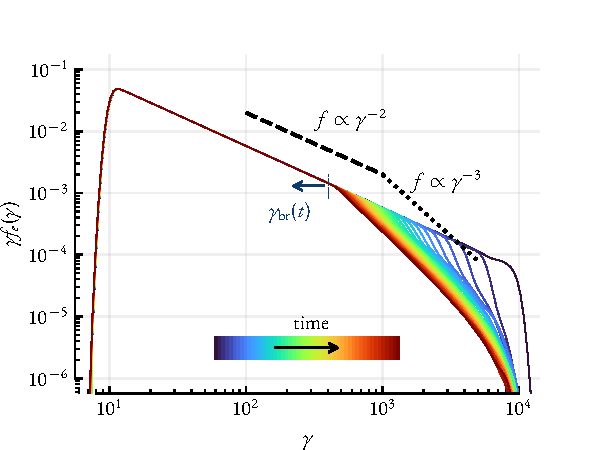
\includegraphics[width=\textwidth]{figures/ch1-numerics/fig_ic.pdf}
    }{
        \caption{Pair plasma (left panel) with an initial temperature of $0.1 m_e c^2$ annihilates producing photons (right panel). These photons interact with plasma via Compton scattering, while also providing new pairs via two-photon pair production. Ultimately a steady state is established with temperature $0.3 m_e c^2$ for the pairs and a corresponding Wien spectrum for photons.}
        \label{fig:num-ic}
    }
\end{figure}

\subsection*{\small \it Emission of photons}

In certain scenarios we might be also interested to study the dynamics of the emitted light. Thus, \texttt{Tristan-MP v2} has a capability of tracking the emitted photons, which are modeled as massless and chargless macroparticles with a trivial equation of motion. These photons are self-consistently emitted by charged particles, that are subject to the radiation reaction force \eqref{eq:num-radiation}, while simultaneously conserving both the energy and momentum of the whole system (particle + emitted photons). The energy of each individual photon radiated by a particle with $\bm{u}=\gamma\beta$ is set by two dimensionless parameters, $\tilde{\gamma}_{\rm syn}$ and $\tilde{\gamma}_{\rm IC}$, in synchrotron and IC case correspondingly:

\begin{equation}
    \begin{aligned}
        \varepsilon_{\rm syn} &= m_e c^2 \chi_R\frac{\gamma^2}{\tilde{\gamma}_{\rm syn}^2},\\
        \varepsilon_{\rm IC} &= m_e c^2 \frac{\gamma^2}{\tilde{\gamma}_{\rm IC}^2}.
    \end{aligned}
\end{equation}
\noindent where $\chi_R$ was defined in \eqref{eq:num-kappa-chi}. Given the photon energies, the emission probability is then chosen in such a way as to preserve the energy and momentum. In IC case the meaning of $\tilde{\gamma}_{\rm IC}$ is rather simple: it determines the energy of photons, $\varepsilon_{\rm rad}$, in the background photon field. Or in other words, particles with $\gamma=\tilde{\gamma}_{\rm IC}$ upscatter photons of energy $\varepsilon_{\rm rad}$ to $m_e c^2$. In synchrotron case $\tilde{\gamma}_{\rm syn}$ corresponds to the energy of particles whose peak synchrotron energy is equal to $m_e c^2$.\footnote{This parameter in practice defines the $\hbar$ in a dimensionless way.} For particles with $\gamma\sim \tilde{\gamma}_{\rm syn}$ the synchrotron peak frequency $\hbar \omega_B \gamma^2$ is equal to $m_e c^2$ (where $\omega_B = |q_e| B_{\rm rad} / m_e c$). These two dimensionless parameters, $\tilde{\gamma}_{\rm syn}$ and $\tilde{\gamma}_{\rm IC}$, are then defined in the following way

\begin{equation}
\begin{aligned}
    \tilde{\gamma}_{\rm syn}^2 &= m_e c^2 / \left(\frac{3}{2}\frac{\hbar |q_e| B_{\rm rad}}{m_e c}\right),\\
    \tilde{\gamma}_{\rm IC}^2 &= m_e c^2 / \varepsilon_0. 
\end{aligned}
\end{equation}

To recap, there are four free dimensionless parameters in total that couple the radiative processes to the plasma physics: $\gamma_{\rm syn}$ and $\tilde{\gamma}_{\rm syn}$ for synchrotron cooling, and $\gamma_{\rm IC}$ and $\tilde{\gamma}_{\rm IC}$ for the inverse-Compton cooling. In real astrophysical systems $\gamma_{\rm IC}$ and $\tilde{\gamma}_{\rm IC}$ depend entirely on the energy density and the peak energy of the background photon field. $\gamma_{\rm syn}$ and $\tilde{\gamma}_{\rm syn}$, on the other hand, are determined by the strength of the magnetic field, $B_{\rm rad}$:

\begin{equation}
    \gamma_{\rm syn}^2\equiv \frac{3 f_{\rm rec}}{2}\frac{B_{\rm cl}}{B_{\rm rad}},~~~\tilde{\gamma}_{\rm syn}^2 = \frac{B_S}{B_{\rm rad}},
\end{equation}

\noindent where $B_{\rm cl} = m_e^2 c^4 / e^3$ is the classical magnetic field, and $B_S = m_e^2 c^3 / e \hbar$ is the Schwinger field. As mentioned earlier, these parameters determine the dynamic importance of cooling (either synchrotron or IC) for particles of different energies. When down-/upscaling the values for these parameters in numerical simulations it is, thus, essential to respect their proper hierarchy with respect to other dimensionless scales.

\section{Two-photon pair-production/-annihilation and Compton scattering}
\label{sec:num-QED}

In some systems, such as the magnetospheres of neutron stars or the coronae of black hole accretion disks, the energetic photons emitted by accelerated charged particles can interact with each other, producing $e^\pm$-plasma in a QED process known as the \emph{Breit-Wheeler pair production} \citep[see, e.g.,][]{1987MNRAS.227..403S, 1996A&A...311..172L, 2017ApJ...850..141B, 2020arXiv201107310B}. The opposite is also true: if the density of pair-plasma is large-enough, electrons and positrons may \emph{annihilate} producing photons. High-energy photons can also Compton scatter on charged particles producing recoil and potentially coupling plasma with radiation.\footnote{IC radiation drag described in previous section is a special case of the same process, except there we do not track the seed photons, assuming them to be uniformly and isotropically distributed.} Including these processes in PIC simulations is, thus, important in order to study their effect on plasma physics self-consistently. In this section we will assume that all the macroparticle weights are equal to $1$, and when an interaction occurs -- initial particles are removed. However, the actual implementation in the \texttt{Tristan-MP v2} code is agnostic to particle weights. 

Consider a process where particles of species $A_1$ and $B_1$ interact producing two other particles, $A_2$ and $B_2$: $A_1+B_1\to A_2+B_2$.\footnote{For instance, in case of the two-photon pair production $A_1$ and $B_1$ are the photons, while $A_2$ and $B_2$ are the electron and the positron.} This processes conserves both the total energy and momentum, and is described by a differential cross-section $d\sigma_{12} / d\Omega$ which determines the angular probability distribution for the momenta of resulting particles $A_2$ and $B_2$. The total cross-section, $\sigma_{12}=\int d\Omega \left(d\sigma_{12} / d\Omega\right)$, multiplied by the relative velocity of initial particles, determines the overall probability for this process to occur in unit time; let us denote that as $p_{12}$. For every individual pair, $A_1$ and $B_1$, the process of simulating the interaction is the following:

\begin{algorithm}[H]
    Lorentz-transform to the reference frame where $d\sigma_{12} / d\Omega$ is defined\;
    evaluate $p_{12}$\;
    $rnd =$ random number $[0;1)$\;
    \If{rnd $\geq p_{12}$}{
        evaluate the total energy and momentum\;
        remove particles $A_1$ and $B_1$\;
        evaluate $f(\theta, \phi) = d\sigma_{12} / d\Omega / \sigma_{12}$\; 
        \tcc {notice that $\int f(\theta,\phi)d\Omega = 1$}
        generate random angles $\theta$ and $\phi$ that satisfy the $f(\theta,\phi)$ probability distribution\;
        evaluate the new momenta for $A_2$ and $B_2$ given $\theta$ and $\phi$ and energy/momentum conservation\;
        create particles $A_2$ and $B_2$\;
        Lorentz-transform back to the lab frame\;
    }
\end{algorithm}

\noindent Formulae for the total and differential cross sections for all of the processes discussed above are given in the appendix~\ref{appendix:num-crosssections}. In practice, it is convenient to renormalize $p_{12}$ and express it in terms of the dimensionless optical depth:
\begin{equation}
    p_{12} = \tau_{T} \frac{\sigma_{12}}{\sigma_T} \frac{1}{n_T} c \Delta t,
\end{equation}
\noindent where $n_T$ is some fiducial density, and $\tau_T$ is the effective optical depth. If a particle $A_1$ is flying with the speed of light through a cloud of other particles with the number density $n_T$ and has an equal cross section of $\sigma_{12}=\sigma_T$ for interacting with either of them, then $\tau_T$ determines its effective optical depth. 

The complication to include the described algorithm in PIC simulations is that all of these processes (two-photon pair production, electron-positron annihilation and Compton scattering) are ``two-body'', and their numerical treatment scales as $\mathcal{O}(N^2)$ with the number of interacting particles, $N$. In \texttt{Tristan-MP v2} we employ a novel Monte Carlo pairing technique, that alleviates this issue and reduces the complexity to $\mathcal{O}(N)$. This algorithm is applicable to all of the above-mentioned processes, and is similar to what is used by the plasma physics community to model Coulomb collisions in PIC codes \citep[see, e.g.,][]{2009shin.confE.163D}. A version of this technique has also been implemented in the \texttt{Osiris} PIC code \citep{2020JPlPh..86e9016D}.

First of all, macroparticles of different species in our simulation are grouped into localized patches in space, called \emph{tiles}; only particles within the same tile are allowed to interact. We then count the number of particles in each tile, $N_t$ (which is typically much less than the number of particles in the whole domain, $N$), and the volume of each tile, $V_t$. Particles within the same tile are then randomly paired with each other (once per timestep). Then the above-mentioned interaction routine is applied, except that the binary probabilities for each of the pairs, $p_{12}$, are multiplied by $N_t / V_t$ to properly recover the optical depth, $\tau_T$.\footnote{Notice, however, that this pairing algorithm is only valid in the limit when $p_{12}\ll N_t^{-1}\ll 1$.}

We further suggest several simplified numerical experiments to verify these algorithms and compare their results with analytic predictions. To test the two-photon pair production we initialize two isotropic and uniform clouds of monoenergetic photons with energies, correspondingly, $\varepsilon_1 = 0.1m_e c^2$ and $\varepsilon_2 = 100 m_e c^2$. As these photon populations interact and pair-produce, we measure the energy distribution function of produced pairs $f_{\pm}(\gamma)$ (Figure~\ref{fig:num-bwpp} and compare it with analytical prediction by \cite{1983Ap.....19..187A}. Notice that as expected particles are only produced in the range of energies $\gamma_{\rm min}<\gamma<\gamma_{\rm max}$, where

\begin{equation}
    m_e c^2 \gamma_{\rm max/min} = \frac{\varepsilon_1 + \varepsilon_2}{2} \pm \frac{\varepsilon_1 - \varepsilon_2}{2}\sqrt{1 - \frac{(m_ec^2)^2}{\varepsilon_1\varepsilon_2}}.
\end{equation}

\begin{figure}[htb]
    \sidebysidecaption{0.555\linewidth}{0.42\linewidth}{
        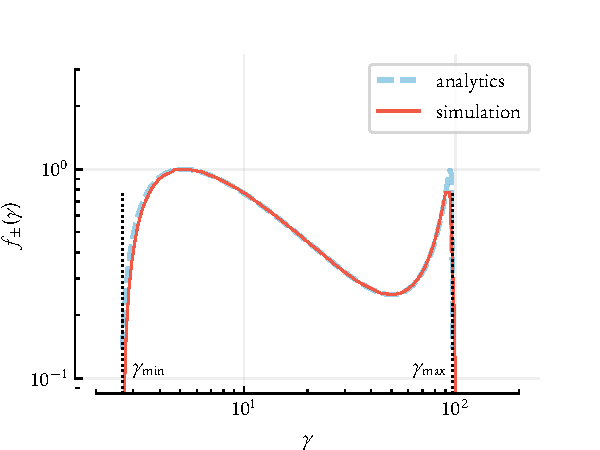
\includegraphics[width=\textwidth]{figures/ch1-numerics/fig_bwpp.pdf}
    }{
        \caption{Distribution of produced $e^\pm$ pairs during the interaction of two isotropic clouds of photons with energies $0.1 m_e c^2$ and $100 m_e c^2$; figure compares analytical prediction with simulations. Analytical expression is provided by \cite{1983Ap.....19..187A}.}
        \label{fig:num-bwpp}
    }
\end{figure}

We test Compton scattering algorithm with a numerical experiment described initially by \cite{1957JETP....4..730K}. A thermal background of electrons and positrons is initialized with a temperature $T_e$. This background then interacts with a monoenergetic beam of photons with energies $\ll m_e c^2$, and thermal equilibrium is established; the emerging photon distribution $f_\gamma \propto \varepsilon^2\exp{-\varepsilon/T_e}$. This process is demonstrated in Figure~\ref{fig:num-kompaneets}, where we plot time-evolving photon spectrum as they approach thermal equilibrium with the background plasma.

\begin{figure}[htb]
    \sidebysidecaption{0.45\linewidth}{0.5\linewidth}{
        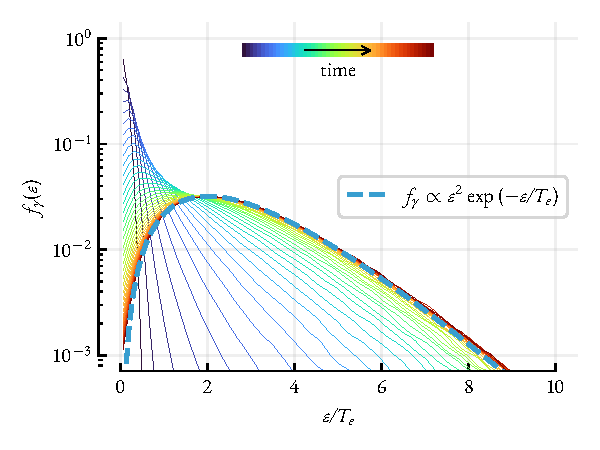
\includegraphics[width=\textwidth]{figures/ch1-numerics/fig_kompaneets.pdf}
    }{
        \caption{Soft background photons thermalizing over time with a bath of electron-positron pairs via Compton scattering, \cite{1957JETP....4..730K}. At late times (red lines) photons are in a thermal equilibrium with plasma.}
        \label{fig:num-kompaneets}
    }
\end{figure}

To test all of the QED effects together we perform another numerical experiment described by \cite{2020arXiv201107310B}. In this case particles can interact via two-photon pair production, pair annihilation, and Compton scattering. Simulation domain is initialized with a thermal background of electrons with a temperature of $T_{\rm init}=0.1 m_e c^2$ and no photons. As particles annihilate, they radiate photons. These photons then attempt to thermalize with the pair-plasma via Compton scattering, while at the same time producing additional pairs via two-photon pair production. The system ultimately reaches the steady state, where plasma is heated to $T_{\rm eq}\approx 3T_{\rm init}$, while the photons are just partially thermalized, forming a Wien spectrum of $f\propto \varepsilon^2\exp{(-\varepsilon/T_{\rm eq})}$. Time evolution of plasma and photon distributions is shown in Figure~\ref{fig:num-svensson}.

\begin{figure}[htb]
    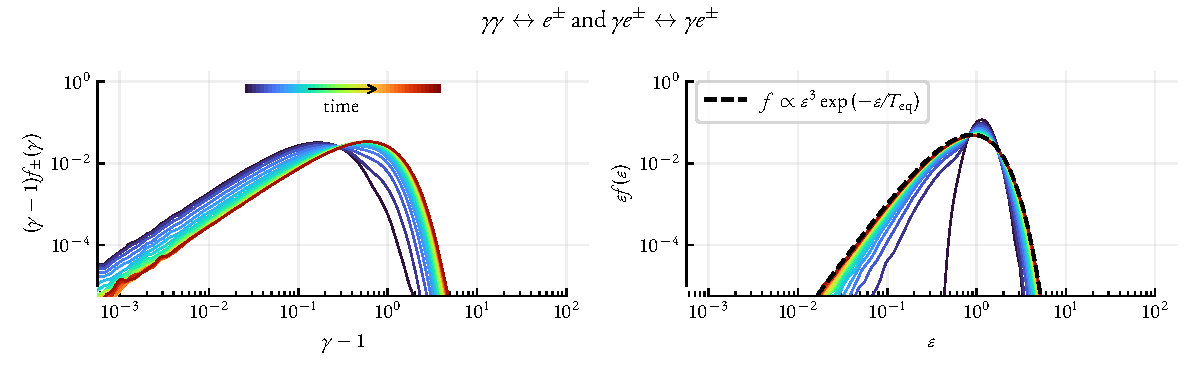
\includegraphics[width=\textwidth]{figures/ch1-numerics/fig_svensson.pdf}
    \caption{Pair plasma (left panel) with an initial temperature of $0.1 m_e c^2$ annihilates producing photons (right panel). These photons interact with plasma via Compton scattering, while also providing new pairs via two-photon pair production. Ultimately a steady state is established with temperature $0.3 m_e c^2$ for the pairs and a corresponding Wien spectrum for photons.}
    \label{fig:num-svensson}
\end{figure}

